\newpage
\section{Auswertung}
\label{sec:Auswertung}
\subsection{Energiebilanz der Anlage und äußere Leistungszahl}
In diesem Teil werden die Leistungszahlen und die Energiebilanz der Anlage berechnet.
\subsubsection{Prüfen Sie die im Bedienmodul angegebene Heizleistung anhand Vor- und Rücklauftemperatur und Heizdurchfluss}
\label{subsubsec:Heizleistung}
Die Heizleistung lässt sich mit der folgenden Formel berechnen:
\begin{equation}
\dot Q_{Kond}= \dot m \cdot cp_{W} \cdot (T_{V} - T_{R})
\label{eq:110623_Heizleistung}
\end{equation}
Mit einem Massenstrom von 0,38 $\frac{kg}{s}$, einer Vorlauftemperatur von 48°C und Rücklauftemperatur von 43°C im Kondensator ergibt sich daraus mit Formel \ref{eq:110623_Heizleistung} eine Heizleistung von 8,14 $\frac{kJ}{s}$ bzw $kW$. Wobei auf dem Display eine Heizleistung von 8,3kW angezeit wird, was nur minimal von unserem errechneten Wert abweicht.
\subsubsection{Berechnen Sie die äußere Leistungszahl der Anlage}
Die tatsächliche äußere Leistungszahl berechnet sich wie in Formel \ref{eq:110623_aeußere Leistungszahl_tatsächlich} dargestellt und beträgt 3,53.
\begin{equation}
\epsilon_{real,a} = \frac{\dot Q_{Nutz}}{P_{el}}
\label{eq:110623_aeußere Leistungszahl_tatsächlich}
\end{equation}
\subsubsection{Berechnen Sie aus der Gesamt-Energiebilanz der Anlage den aus der Umgebung aufgenommenen Wärmestrom im Verdampfer.
Welcher Luftvolumenstrom muss durchgesetzt werden, wenn die Luft um 5 K abgekühlt wird?}
Um den aus der Umgebung aufgenommenen Wärmestrom zu bestimmen muss die Gesammt-Energiebilanz der Anlage verwendet werden:
\begin{equation}
\dot Q_{Verd}=\dot Q_{Verd}-P_{el}
\label{eq:110623_aeußere Leistungszahl}
\end{equation}
Mit der berechneten Heizleistung von 8,14kW und einer elektrischen Leistung von 2304W ergibt sich ein vom Verdampfer aufgenommerner Wärmestrom von 5,84kW. Nun wird der benötigte Luftstrom, unter der Annahme, dass die durchströmende Luft um 5K abgekühlt wird, berechnet.
\begin{equation}
\dot V_{L}=\frac{\dot Q_{verd}}{\rho_{Luft} \cdot cp_{Luft} \cdot \Delta T}
\label{eq:110623_benoetigter_Luftstrom}
\end{equation}
Der benötigte Luftstrom beträgt nach Formel \ref{eq:110623_benoetigter_Luftstrom} 1,36$\frac{m^3}{s}$. 
\subsubsection{Berechnen Sie die äußere Carnot-Leistungszahl der Anlage \texorpdfstring{$\epsilon_{Carnot,a}$}{} anhand der erreichten Mitteltemperatur der Nutzwärme TmN =(TKessel + TRück )/2 und der Umgebungstemperatur.}
Für die äußere Carnot-Leistungszahl der Anlage benötigt man die Umgebungstemperatur $T_{U}=$24°C und die mittlere Temperatur der Nutzwärme $T_{mN}=$48,25°C. Die äußere Carnot-Leistungszahl berechnet sich dann wie folgt: 
\begin{equation}
\epsilon_{Carnot, Außen} = \frac{T_{mN}}{T_{mN}-T_{U}}
\label{eq:110623_aeußere Carnot Leistungszahl}
\end{equation}
Sie beläuft sich dabei auf 13,25.

\subsection{Arbeitsmittelkreislauf und innere Leistungszahlen}
Entsprechend der Werte aus Messreihe 1, welche in \autoref{tab:Arbeitspunkte} zusammengefasst sind, kann das passende
lg(p)-h-Diagramm, mit den Arbeitspunkten 1-4 erstellt werden. Aus diesem Diagramm lassen sich die in \autoref{tab:Arbeitspunkte} ebenfalls
notierten Enthalpien ablesen.

\begin{table}[!h]
    \centering
    \resizebox{\textwidth}{!}{%
    \begin{tabular}{|c|c|c|c|}
    \hline
    \multicolumn{1}{|l|}{Arbeitspunkt} & Bezeichnung                  & \multicolumn{1}{l|}{Temperatur in °C} & \multicolumn{1}{l|}{Enthalpie in kJ/kg} \\ \hline
    1                                  & Temperatur nach Verdampfer   & 18                                    & 425                                     \\ \hline
    2                                  & Heißgastemperatur            & 63                                    & 448                                     \\ \hline
    3                                  & Temperatur nach Verflüssiger & 43                                    & 280                                     \\ \hline
    4                                  & Temperatur vor Verdampfer    & 16                                    & 280                                     \\ \hline
    \end{tabular}%
    }
    \caption{Arbeitspunkte entsprechend Messreihe 1}
    \label{tab:Arbeitspunkte}
    \end{table}

    Zusätzlich kann das obere Druckniveau von 29,5 bar und das unter Druckniveau von rund 13 bar abgelesen werden.
    Des Weiteren ist in \autoref{fig:lgp-h-Diagramm} ersichtlich, dass die Ergebnisse plausibel sind, da der dargestellte Kreisprozess dem erwarteten Bild entspricht.\\

    \begin{figure}[!h]
        \centering
        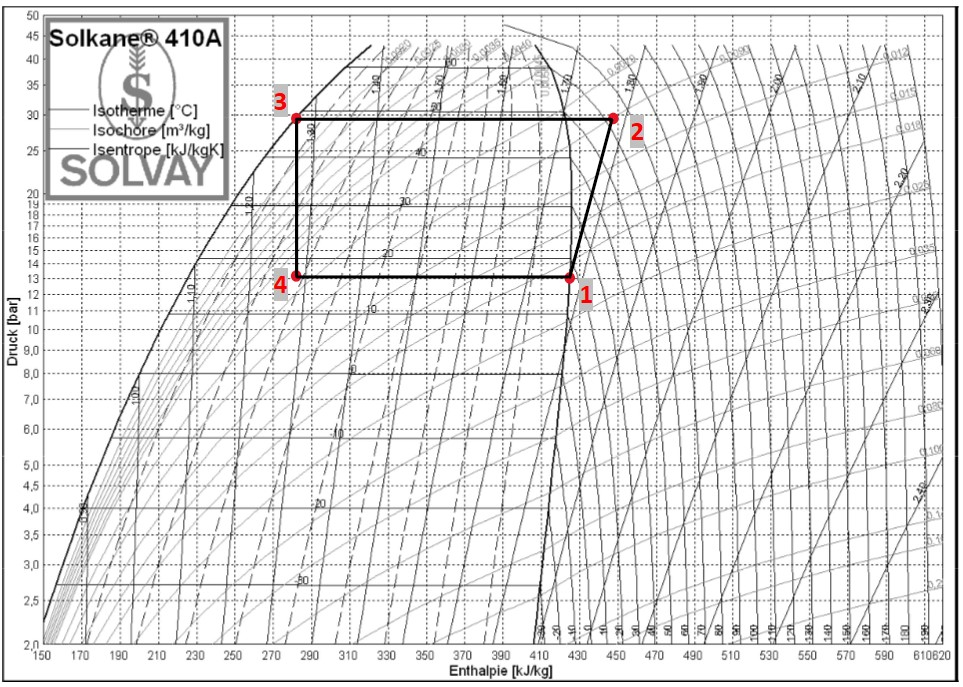
\includegraphics[width=0.5\textwidth]{Abbildungen/lgp-h-diagramm.jpg}
        \caption{lg(p)-h-Diagramm mit den Arbeitspunkten aus Messreihe 1}
        \label{fig:lgp-h-Diagramm}
    \end{figure}

Mit den Temperaturen aus \autoref{tab:Arbeitspunkte} kann mittels \autoref{eq:Innere Carnot-Leistungszahl} die innere Carnot-Leistungszahl
ermittelt werden. Die Berechnung ergibt dann eine innere Carnot-Leistungszahl von 7,15.

    \begin{equation}
        \epsilon_{Carnot, Innen}=\frac{T_{max}}{T_{max}-T_{min}}=\frac{T_{Kond}}{T_{Kond}-T_{Verd}}=\frac{336,15 K}{336,15 K-289,15 K}=7,15
        \label{eq:Innere Carnot-Leistungszahl}
    \end{equation}

 In \autoref{fig:lgp-h-Diagramm-is} ist zusätzlich der isentrope Arbeitspunkt 2 eingezeichnet und somit die isentrope Enthalpie für diesen Arbeitspunkt von $440 \frac{kJ}{kg}$
 eingezeichnet und abzulesen.
    
 \begin{figure}[!h]
        \centering
        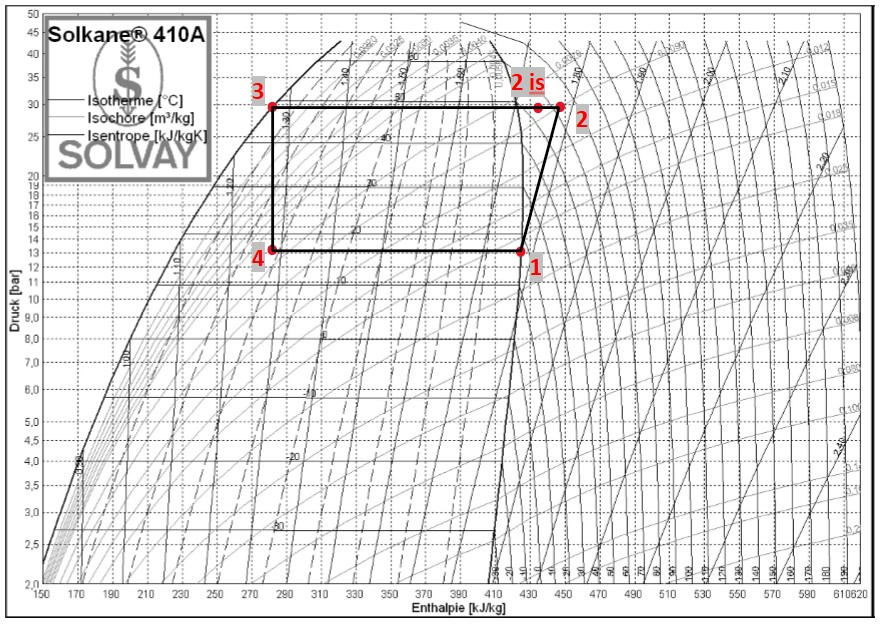
\includegraphics[width=0.5\textwidth]{Abbildungen/lgp-h-diagramm-is.jpg}
        \caption{lg(p)-h-Diagramm mit dem isentropen Arbeitspunkt 2}
        \label{fig:lgp-h-Diagramm-is}
    \end{figure}

    Mittels der nun bekannten isentropen Enthalpie für Arbeitspunkt 2 kann mittels \autoref{eq:Isentropenwirkungsgrad} der Isentropenwirkungsgrad ermittelt werden.
\begin{equation}
    \eta_{is}=\frac{h_{2,is}-h_{1}}{h_{2}-h_{1}}=\frac{433 kJ/kg-425 kJ/kg}{448 kJ/kg-425 kJ/kg}=0,6521
    \label{eq:Isentropenwirkungsgrad}
\end{equation}

Der Isentropenwirkungsgrad für diesen Fall beträgt demnach 0,6521.\\


\subsection{Leistungszahlen und Verlustursachen}

\subsection{Energiebilanzen Einzelapparate}

\subsubsection{} 
\label{subsec:Massenstrom}

\subsubsection{}
\subsubsection{Der Durchmesser der Heißgasleitung beträgt 16 mm, der der Kondensatleitung 10
mm. Berechnen Sie mit Hilfe der aus Diagramm bzw. Dampftafel abgelesenen spezifischen Volumina die Strömungsgeschwindigkeiten von Gas und Flüssigkeit.}

Das spezifische Volumen des Gases kann aus dem lg(p)-h Diagramm abgelesen werden zu: $V_{Gas}=0,02 m^3/kg$. Die Dichte, welche der Kehrwert des spezifischen Volumens ist, ergibt sich als $\rho=50 kg/m^3$. 
Mit dem durchschnittlichen Massenstrom aus \autoref{subsec:Massenstrom} können die Strömungsgeschwindigkeiten über den Volumenstrom nach folgenden Gleichungen berechnet werden.

\begin{equation}
    \dot{V}= \frac{\dot{m}}{\rho }
    \label{eq:230620_Volumenstrom}
\end{equation}

\begin{equation}
    \dot{V}= v \cdot \frac{\pi}{4} \cdot d^2
    \label{eq:230620_Volumenstrom2}
\end{equation}

Werden \autoref{eq:230620_Volumenstrom} und \autoref{eq:230620_Volumenstrom2} gleichgesetzt ergibt sich die Strömungsgeschwindigkeit nach \autoref{eq:230620_Strömungsgeschwindigkeiten}.

\begin{equation}
    v = \frac{\dot{m}}{\frac{\pi}{4}\cdot \rho \cdot d^2}
    \label{eq:230620_Strömungsgeschwindigkeiten}
\end{equation}

Am Arbeitspunkt 1 ergibt sich die Strömungsgeschwindigkeit:
$$v=\frac{0,0444 kg/s}{\frac{\pi}{4}\cdot 50 kg/m^3 \cdot (0,016 m)^2}=4,42 m/s $$

Der Druck am Arbeitspunkt 3 kann aus dem lg(p)-h Diagramm als $p=30 bar$ abgelesen werden. Mithilfe dessen lässt sich die Dichte aus der Dampftafel als $\rho=914,34 kg/m^3$ bestimmen.
Die Strömungsgeschwindigkeit der Flüssigkeit am Arbeitspunkt 3 berechnet sich dann zu:
$$v=\frac{0,0444 kg/s}{\frac{\pi}{4}\cdot 914,37 kg/m^3 \cdot (0,01 m)^2}=0,618 m/s $$

\subsubsection{Skizzieren Sie ein T,A-Schaubild des kleinen Gegenstrom-Plattenwärmeübertragers
zwischen internem und externem Heizkreis. Berechnen Sie den erreichten k-Wert,
wenn der Apparat eine Wärmeübertragerfläche eine Fläche von \texorpdfstring{$A = 0,4 m^2$}{} hat.}

\begin{figure}[!h]
    \centering
    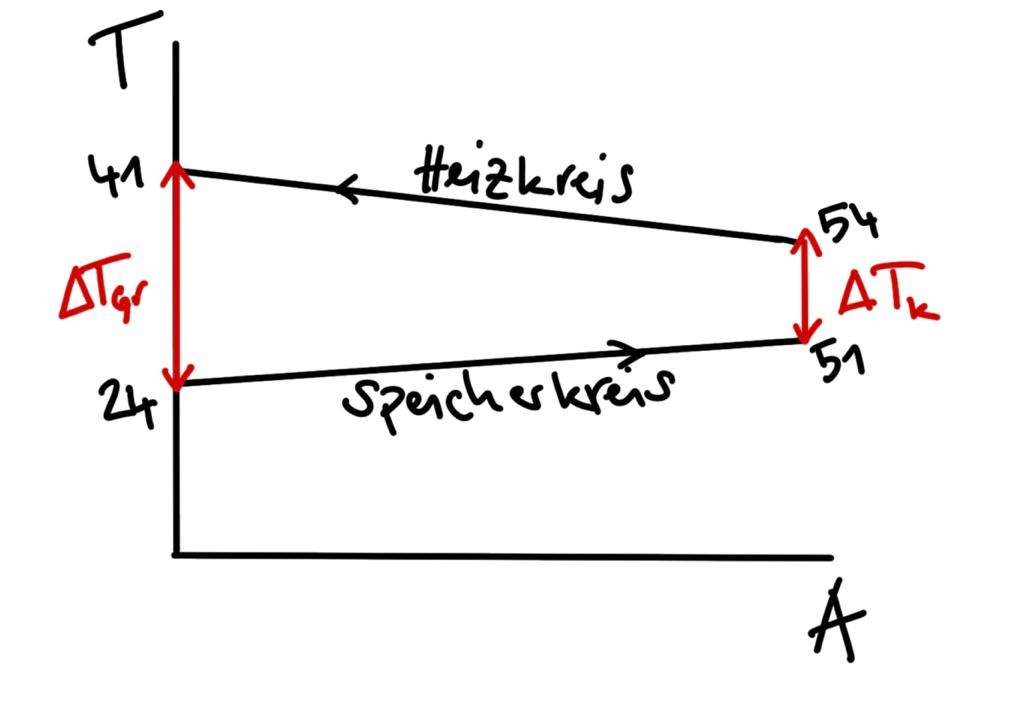
\includegraphics[width=0.5\textwidth]{Abbildungen/TA,Diagramm.jpeg}
    \caption{T,A-Schaubild eines Gegenstrom-Plattenwärmeübertragers}
    \label{fig:TA,Diagramm}
\end{figure}

NOCHMAL NEU ZEICHNEN!!!!

Für die Berechnung des K-Wert muss im Vorfeld $\Delta T_M$ bestimmt werden. Das passiert nach folgender Gleichung.

\begin{equation}
    \Delta T_{MAX}= \Delta T_{HA}-\Delta T_{KE}
    \label{eq:230621_DeltaTMAX}
\end{equation}

$$\Delta T_{MAX}= 41°C-24°C= 17K$$

\begin{equation}
    \Delta T_{MIN}= \Delta T_{HE}-\Delta T_{KA}
    \label{eq:230621_DeltaTMIN}
\end{equation}

$$\Delta T_{MIN}= 54°C-51°C= 3K$$

\begin{equation}
    \Delta T_{M}= \frac{\Delta T_{MAX}-\Delta T_{MIN}}{ln\frac{\Delta T_{MAX}}{\Delta T_{MIN}}}
    \label{eq:230621_DeltaTM}
\end{equation}

$$\Delta T_M= \frac{17K-3K}{ln\frac{17K}{3K}}= 8,07K$$

Mithilfe der \autoref{eq:230621_Q} und der Heizleistung lässt sich der k-Wert bestimmen.

\begin{equation}
    \dot{Q}=k\cdot A \cdot \Delta T_M
    \label{eq:230621_Q}
\end{equation}

\begin{equation}
    k = \frac{\dot{Q}}{ A \cdot \Delta T_M} 
    \label{eq:230621_k}
\end{equation}

$$k=\frac{8,14 kW}{ 0,4m^2 \cdot 8,07K}=6,3 kW/m^2K$$

\subsubsection{Wie lange dauert es bei konstanter Wärmepumpenleistung, bis ausgehend von einer
konstanten Anfangstemperatur \texorpdfstring{$T_{Sp,U}$}{} der gesamte Speicherinhalt (450 l) aufgeheizt ist?}

Die Wärmemenge die benötigt wird um den Speicher aufzuheizen berechnet sich nach:

\begin{equation}
Q = m \cdot c_p \cdot \Delta T = \rho \cdot V \cdot c_p \cdot \Delta T
\end{equation}

$$Q= 997 kg/m^3 \cdot 0,45 m^3 \cdot 4,18 kJ/kgK (35°C-22°C)K=24,4 MJ$$

Da die Heizleistung nur eine Energieangabe pro Zeiteinheit ist lässt sich die Zeit durch eine einfache Gleichung bestimmen.

\begin{equation}
    P_{Heiz}= \frac{Q}{t}
\end{equation}

\begin{equation}
 t = \frac{Q}{P_{Heiz}}
\end{equation}

$$ t= \frac{24,4 MJ}{8,14 kW}=2995 s= 49,9 min$$